\documentclass[xetex,mathserif,serif]{beamer}
\usepackage{polyglossia}
\setdefaultlanguage[babelshorthands=true]{russian}
\usepackage{minted}
\usepackage{tabu}
\usepackage{moresize}

\useoutertheme{infolines}

\usepackage{fontspec}
\setmainfont{FreeSans}
\newfontfamily{\russianfonttt}{FreeSans}

\definecolor{links}{HTML}{2A1B81}
\hypersetup{colorlinks,linkcolor=,urlcolor=links}

\setbeamertemplate{blocks}[rounded][shadow=false]

\setbeamercolor*{block title alerted}{fg=red!50!black,bg=red!20}
\setbeamercolor*{block body alerted}{fg=black,bg=red!10}

\tabulinesep=1.2mm

\title{Многопоточное программирование}
\subtitle{Практика}
\author[Юрий Литвинов]{Юрий Литвинов\\\small{\textcolor{gray}{yurii.litvinov@gmail.com}}}
\date{20.09.2019г}

\newcommand{\attribution}[1] {
\vspace{-2mm}\begin{flushright}\begin{scriptsize}\textcolor{gray}{\textcopyright\, #1}\end{scriptsize}\end{flushright}
}

\newcommand{\DownArrow} {
	\hspace{2cm}\begin{LARGE}$\downarrow$\end{LARGE}
}

\begin{document}

	\frame{\titlepage}

	\section{Задача}

	\begin{frame}
		\frametitle{Задача, ``Обедающие философы''}
		\begin{columns}
			\begin{column}{0.5\textwidth}
				\begin{itemize}
					\item Есть N тарелок спагетти, N вилок и N философов
					\item Философ может думать и есть
					\item Чтобы есть, философу нужны две вилки
					\item Пример --- транзакция, переводящая деньги со счёта на счёт
				\end{itemize}
			\end{column}
			\begin{column}{0.5\textwidth}
				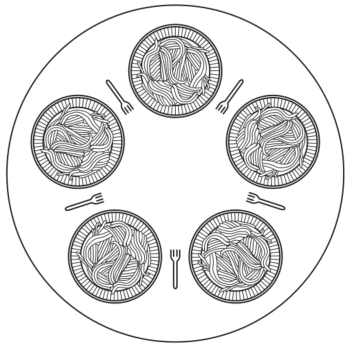
\includegraphics[width=0.9\textwidth]{diningPhilosophers.png}
				\attribution{A. Tanenbaum, Modern Operating Systems}
			\end{column}
		\end{columns}
	\end{frame}

	\begin{frame}
		\frametitle{Что надо сделать}
		\begin{itemize}
			\item Смоделировать ситуацию обедающих философов
			\begin{itemize}
				\item Придумать красивую объектно-ориентированную модель
			\end{itemize}
			\item Выводить на экран состояния философов
			\item Считаем, что философы думают и едят случайное, но небольшое количество времени
			\item Реализация должна гарантировать отсутствие взаимоблокировок
			\item Нужны юнит-тесты, проверяющие, что если философы известно как думают и едят, никто не останется голодным
		\end{itemize}
	\end{frame}

\end{document}
